%!TEX output_directory = temp
\documentclass[letterpaper, 12pt]{amsart}
	%%%%%%%%%%%%%%%%%%%%%%%%%%%%%%%%%%%%%%%%%%%%%%%%%%%%%%%%%%%%%%%%%%%%%%%%%%%%%%
	%%%%%%%%%%%%%%%%%%%%%%%%%%%% boilerplate packages %%%%%%%%%%%%%%%%%%%%%%%%%%%%
	\usepackage{amsmath,amssymb,amsthm}
	\usepackage[mathscr]{euscript}
	\usepackage{enumerate}
	\usepackage{graphicx}
	\usepackage{mathrsfs}
	\usepackage{color}
	\usepackage{hyperref}
	\usepackage{verbatim}
	\usepackage{stmaryrd}
	\usepackage[margin=1.25in]{geometry}

	\raggedbottom

	%%%%%%%%%%%%%%%%%%%%%%%%%%%%%%%%%%%%%%%%%%%%%%%%%%%%%%%%%%%%%%%%%%%%%%%%%%%%%%
	%%%%%%%%%%%%%%%%%%%%%%%%%%%%% rename the abstract %%%%%%%%%%%%%%%%%%%%%%%%%%%%
	% \renewcommand{\abstractname}{Introduction}

	%%%%%%%%%%%%%%%%%%%%%%%%%%%%%%%%%%%%%%%%%%%%%%%%%%%%%%%%%%%%%%%%%%%%%%%%%%%%%%
	%%%%%%%%%%%%%%%%%%%%%%%%%%%%%%%%%%%%% sets %%%%%%%%%%%%%%%%%%%%%%%%%%%%%%%%%%%
		%% sets 
		\DeclareMathOperator{\N}{\mathbb{N}}
		\DeclareMathOperator{\Z}{\mathbb{Z}}
		\DeclareMathOperator{\Zp}{\mathbb{Z}^{+}}
		\DeclareMathOperator{\Q}{\mathbb{Q}}
		\DeclareMathOperator{\Qp}{\mathbb{Q}^{+}}
		\DeclareMathOperator{\Qc}{\mathbb{Q}^{c}}
		\DeclareMathOperator{\R}{\mathbb{R}}
		\DeclareMathOperator{\F}{\mathbb{F}}
		\DeclareMathOperator{\Rp}{\mathbb{R}^{+}}
		\DeclareMathOperator{\C}{\mathbb{C}}
		\DeclareMathOperator{\Cnon}{\mathbb{C}^{\times}}
		%% powerset of a set
		\DeclareMathOperator{\pset}{\mathcal{P}}
		%% set of continuous functions in a certain variable
		\DeclareMathOperator{\cont}{\mathscr{C}}
		%% set of functions in a certain variable
		\DeclareMathOperator{\func}{\mathscr{F}}
		
	%%%%%%%%%%%%%%%%%%%%%%%%%%%%%%%%%%%%%%%%%%%%%%%%%%%%%%%%%%%%%%%%%%%%%%%%%%%%%%
	%%%%%%%%%%%%%%%%%%%%%%%%%%%%%%%% linear algebra %%%%%%%%%%%%%%%%%%%%%%%%%%%%%%
		%% linear span
		\DeclareMathOperator{\Ell}{\mathscr{L}}
		%% bold vectors with arrows, and bold matrices
		\newcommand{\bmat}[1]{{\mathbf{#1}}}
		\newcommand{\bvec}[1]{{\vec{\mathbf{#1}}}}
		%% independent vectors/matrices
		\DeclareMathOperator{\ind}{\perp\!\!\!\perp}
		%% order
		\DeclareMathOperator{\ord}{\text{ord}}

	%%%%%%%%%%%%%%%%%%%%%%%%%%%%%%%%%%%%%%%%%%%%%%%%%%%%%%%%%%%%%%%%%%%%%%%%%%%%%%
	%%%%%%%%%%%%%%%%%%%%%%%%%%% probability & statistics %%%%%%%%%%%%%%%%%%%%%%%%%
		%% probability, expectation, variance, etc.
		\renewcommand{\Pr}{\mathbb{P}}
		\DeclareMathOperator{\E}{\mathbb{E}}
		\DeclareMathOperator{\var}{\rm Var}
		\DeclareMathOperator{\sd}{\rm SD}
		\DeclareMathOperator{\cov}{\rm Cov}
		\DeclareMathOperator{\SE}{\rm SE}
		\DeclareMathOperator{\ssreg}{{\rm SS}_{{\rm Reg}}}
		\DeclareMathOperator{\ssr}{{\rm SS}_{{\rm Res}}}
		\DeclareMathOperator{\sst}{{\rm SS}_{{\rm Tot}}}

	%%%%%%%%%%%%%%%%%%%%%%%%%%%%%%%%%%%%%%%%%%%%%%%%%%%%%%%%%%%%%%%%%%%%%%%%%%%%%%
	%%%%%%%%%%%%%%%%%%%%%%%%%%%%%%%% congruences %%%%%%%%%%%%%%%%%%%%%%%%%%%%%%%%%
		\renewcommand{\mod}[1]{\ (\mathrm{mod}\ #1)}

	%%%%%%%%%%%%%%%%%%%%%%%%%%%%%%%%%%%%%%%%%%%%%%%%%%%%%%%%%%%%%%%%%%%%%%%%%%%%%%
	%%%%%%%%%%%%%%%%%%%%%%%%%%%%%% bracket notation %%%%%%%%%%%%%%%%%%%%%%%%%%%%%%
		% I first used this for principal ideals, that is why the abbreviation is pid
		\newcommand{\pid}[1]{\langle #1 \rangle}

	%%%%%%%%%%%%%%%%%%%%%%%%%%%%%%%%%%%%%%%%%%%%%%%%%%%%%%%%%%%%%%%%%%%%%%%%%%%%%%
	%%%%%%%%%%%%%%%%%%%%%%%%%%%%%%% fatdot notation %%%%%%%%%%%%%%%%%%%%%%%%%%%%%%
		\makeatletter
			\newcommand*\fatdot{\mathpalette\fatdot@{.5}}
			\newcommand*\fatdot@[2]{\mathbin{\vcenter{\hbox{\scalebox{#2}{$\m@th#1\bullet$}}}}}
		\makeatother

	%%%%%%%%%%%%%%%%%%%%%%%%%%%%%%%%%%%%%%%%%%%%%%%%%%%%%%%%%%%%%%%%%%%%%%%%%%%%%%
	%%%%%%%%%%%%%%%%%%%%%%%%%%%%%% use pretty letters %%%%%%%%%%%%%%%%%%%%%%%%%%%%
		\DeclareMathOperator{\ep}{\varepsilon}
		\DeclareMathOperator{\ph}{\varphi}

	%%%%%%%%%%%%%%%%%%%%%%%%%%%%%%%%%%%%%%%%%%%%%%%%%%%%%%%%%%%%%%%%%%%%%%%%%%%%%%
	%%%%%%%%%%%%%%%%%%%%%%%%%%% stolen from Jeske/Dugger %%%%%%%%%%%%%%%%%%%%%%%%%
	% Some theorem-like environments, all numbered together starting at 1
	% in each section.

	% The default \theoremstyle is bold headings and italic body text.
	\newtheorem{thm}{Theorem}[section]
	\newtheorem{defn}[thm]{Definition}
	\newtheorem{prop}[thm]{Proposition}
	\newtheorem{claim}[thm]{Claim}
	\newtheorem{cor}[thm]{Corollary}
	\newtheorem{lemma}[thm]{Lemma}

	\theoremstyle{definition}  % Bold headings and Roman body text.
	\newtheorem{example}[thm]{Example}
	\newtheorem{examples}[thm]{Examples}
	\newtheorem{exercise}[thm]{Exercise}
	\newtheorem{note}[thm]{Note}
	\newtheorem{remark}[thm]{Remark}
	\newtheorem{remarks}[thm]{Remarks}
	\newtheorem{discussion}[thm]{Discussion}

	\newcommand{\dfn}{\textbf} % Make defined words bold.
	\newcommand{\mdfn}[1]{\dfn{\mathversion{bold}#1}} % Even make math symbols bold

	% Various commands that are useful.  Please add your own.

	\DeclareMathOperator{\Arg}{Arg}
	\DeclareMathOperator{\re}{Re}
	\DeclareMathOperator{\im}{Im}
	\DeclareMathOperator{\Log}{Log}
	\DeclareMathOperator{\Span}{Span}

	\newcommand{\iso}{\cong}						% isometric/congruent
	\newcommand{\ra}{\rightarrow}                   % right arrow
	\newcommand{\Ra}{\Rightarrow}                   % right implies
	\newcommand{\lra}{\longrightarrow}              % long right arrow
	\newcommand{\la}{\leftarrow}                    % left arrow
	\newcommand{\La}{\Leftarrow}                    % left implies
	\newcommand{\lla}{\longleftarrow}               % long left arrow
	\newcommand{\llra}[1]{\stackrel{#1}{\lra}}      % labeled long right arrow
	\newcommand{\we}{\llra{\sim}}                   % weak equivalence
	\newcommand{\cof}{\rightarrowtail}              % cofibration
	\newcommand{\fib}{\twoheadrightarrow}           % fibration
	\newcommand{\inc}{\hookrightarrow}              % inclusion
	\newcommand{\dbra}{\rightrightarrows}           % double arrow for equalizer diagrams
	\newcommand{\eqra}{\llra{\sim}}                 % equivalence/isomorphism

	% \newcommand{\blank}{\underbar{\ \ }}          % An underscore, as in (__)xV
	\newcommand{\blank}{-}                          % A hyphen, as in (-)xV
	\newcommand{\Id}{Id}                            % The identity functor
	\newcommand{\und}{\underline}
	\newcommand{\norm}[1]{\mid \!\!#1 \!\!\mid}             %\norm{x} gives |x|

	% These commands are for the period and comma in the lower right entry of
	% a diagram.  They put the punctuation 2 pts to the right, but make
	% TeX (and hence the diagram package) unaware of the extra width
	% of that entry.
	\newcommand{\period}    {{\makebox[0pt][l]{\hspace{2pt} .}}}
	\newcommand{\comma}     {{\makebox[0pt][l]{\hspace{2pt} ,}}}
	\newcommand{\semicolon} {{\makebox[0pt][l]{\hspace{2pt} ;}}}

	\newcommand{\Cech}{\v{C}ech}
	\newcommand{\scat}{\Delta}
	\newcommand{\assign}{\ra}
	\newcommand{\copr}{\,\amalg\,}
	\newcommand{\ovcat}{\downarrow}
	\newcommand{\pder}[2]{{\frac{\partial #1}{\partial #2}}}
	\newcommand{\del}{\nabla}
	\newcommand{\vectr}[1]{{\mbox{\boldmath $#1$}}}
	\newcommand{\uvectr}[1]{\vectr{\hat #1}}
	\newcommand{\ihat}{\uvectr \imath}
	\newcommand{\jhat}{\uvectr \jmath}
	\newcommand{\khat}{\uvectr k}
	\newcommand{\rhat}{\uvectr r}
	\newcommand{\thhat}{\uvectr \theta}
	\newcommand{\zhat}{\uvectr z}
	\newcommand{\rhohat}{\uvectr \rho}
	\newcommand{\phihat}{\uvectr \phi}
	\newcommand{\grad}{\vectr{\vec\nabla}}
	% \newcommand{\R}{\mathbb{R}}
	\newcommand{\vv}[1]{\vectr{v_{#1}}}
	\newcommand{\crad}{0.1}
	\newcommand{\lline}[1]{\overleftrightarrow{#1}}
	\DeclareMathOperator{\area}{area}
	\DeclareMathOperator{\vol}{vol}
	\newcommand{\ray}[1]{\overset{\rightarrow}{#1}}
	\newcommand{\sr}[2]{???}
	\newcommand{\iihat}{i}
	\newcommand{\jjhat}{j}
	\newcommand{\kkhat}{k}

	\renewcommand{\abstractname}{Comment}		
\begin{document}
	\title{Homework 2  -- Math 397 \\ \today}
	\author{Alex Thies \\ \href{mailto:athies@uoregon.edu}{\lowercase{athies$@$uoregon.edu}}}

	\begin{abstract}
		I was unable to finish this assignment because I was out of town, and off the grid from last Thursday through late Sunday evening.
		I had to skip most of \#2 and \#3.
	\end{abstract}

	\maketitle

	Starting with the parabola y = x2 and a chord AB, our goal will be to compute the area bounded between the parabola and the chord:
	\begin{figure}[h]
		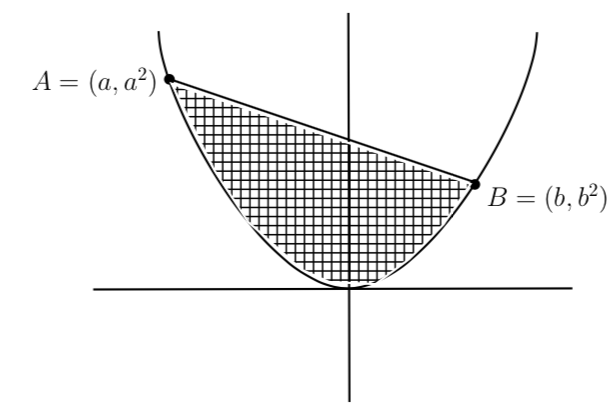
\includegraphics[width=0.4\textwidth]{figures/0.png}
	\end{figure}

	Classically this was known as the ``quadrature of the parabola.'' 
	It was first solved by Archimedes, using the method of exhaustion. 
	In problems 1-3 we will follow his technique but using some modern differential calculus to simplify a few of the hairier geometric steps. 
	We assume $a$ and $b$ as given, with $a < b$. 
	Note that $a$ and $b$ might both be negative, or both positive, in addition to the case shown in the picture. 
	We will let $A$ denote the area we are trying to calculate.

	\section*{Problem 1}
		\subsection*{Part (a)}
		Calculate the slope $\lambda$ of $AB$ in terms of $a$ and $b$, and write down the equation for the line $AB$.

		\begin{proof}[Solution]
		Let the points of intersection between the parabola $y = x^{2}$ and the chord $AB$ be $A = (a, a^{2})$ and $B = (b, b^{2})$, and let the slope of $x^{2}$ be $\lambda$, we compute $\lambda$ (notice the difference of squares):
			\begin{align*}
				\lambda &= \frac{b^{2} - a^{2}}{b - a}, \\
				&= \frac{(b - a)(b + a)}{b - a}, \\
				&= b + a.
			\end{align*}
		Hence, we have $\lambda = a + b$.

		Recall the point-slope form of a line with slope $a$ and point $(x_{1}, y_{1})$: $$y - y_{1} = a(x - x_{1}).$$
		
		Utilizing this we find that chord $AB$ can be written as the line $y = x(a + b) - ab$.
		\end{proof}
		% subsection part_a (end)
	
		\subsection*{Part (b)}
		In the picture 
		\begin{figure}[h]
		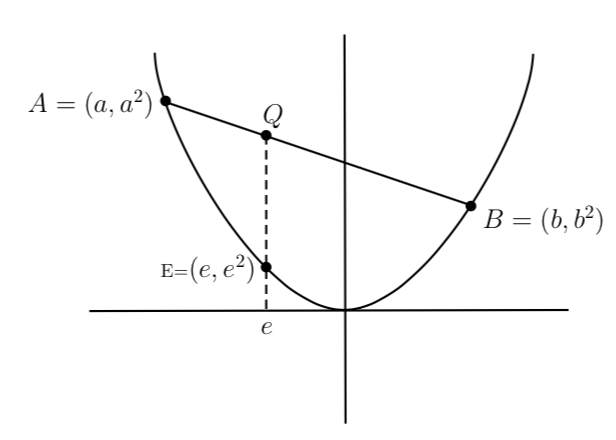
\includegraphics[width=0.4\textwidth]{figures/1.png}
		\end{figure}

		show that the value of $e$ that makes the vertical distance from $E$ to $AB$ (shown as $EQ$ in the picture) as large as possible is $e = a+b$. 
		Do this by writing down the function $d(e)$ that computes this distance and then using calculus to find where it assumes its maximum value.

		\begin{proof}[Solution]
		Recall the distance formula for two points, $P_{1} = (x_{1}, y_{1})$ and $P_{2} = (x_{2}, y_{2})$, in Euclidean space: $$d(P_{1},P_{2}) = \sqrt{(x_{1} - x_{2})^{2} + (y_{1} - y_{2})^{2}}.$$

		We have $E = (e, e^{2})$ on the parabola $y = x^{2}$, let $Q = (e, e(a + b) - ab)$ be the point on chord $AB$ that is on the vertical line $x = e$.
		We will show by maximizing $d(E,Q)$ that $e = (a+b)/2$ is the point on the parabola $x^{2}$ that is farthest away from chord $AB$.
		First, we simplify the distance formula:
			\begin{align*}
				d(E,Q) &= \sqrt{(e - e)^{2} + \left( e^{2} - e(a + b) - ab \right)^{2}}, \\
				&= \sqrt{(0)^{2} + \left( e^{2} - e(a + b) - ab \right)^{2}}, \\
				&= \sqrt{\left( e^{2} - e(a + b) - ab \right)^{2}}, \\
				&= e^{2} - e(a + b) - ab.
			\end{align*}
		We now optimize $d(E,Q)$:
			\begin{align*}
				\frac{d}{de}\left[ e^{2} - e(a + b) - ab \right] &= 0, \\
				2e - a - b &= 0, \\
				2e &= a + b, \\
				e &= \frac{a + b}{2}.
			\end{align*}
		Notice that $d''(E,Q) > 0$, hence $e = (a + b)/2$ is a maximum. 
		Hence, we confirm that the $x$-value which maximizes the distance between the parabola $x^{2}$ and the chord $AB$ is $x = e = (a + b)/2$; we denote this point $E = (e, e^{2})$.
		\end{proof}
		% subsection part_b (end)

		\subsection*{Part (c)}
		In the picture 
		\begin{figure}[h]
		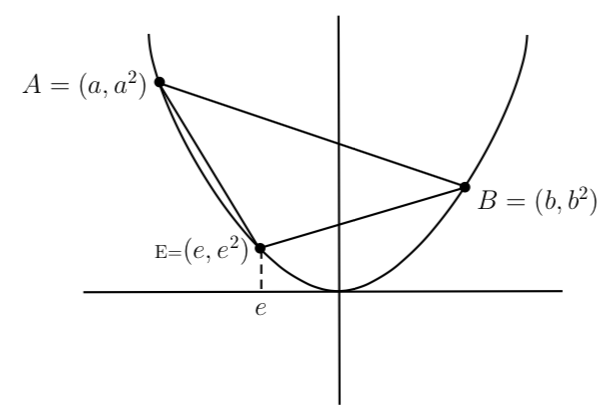
\includegraphics[width=0.4\textwidth]{figures/2.png}
		\end{figure}

		show that the value of $e$ that makes the area of $\triangle ABE$ as large as possible is also $e = a+b$. 
		Compute that this largest area is $\frac{1}{8}(b - a)^{3}$.
		Hint: If $\bvec{v} =(v_{1}, v_{2})$ and $\bvec{w} = (w_{1}, w_{2})$, then the absolute value of $\det 􏰃\begin{bmatrix} v_{1} & v_{2} \\ w_{1} & w_{2}	\end{bmatrix}$ is the area of the parallelogram whose sides are the vectors $\bvec{v}$ and $\bvec{w}$.
		So for a triangle with vertices $(u, v)$, $(x, y)$, $(z, w)$, the area can be computed as $$\left| \frac{1}{2} \det \begin{bmatrix} x - u & y - v \\ z - u & w - v \end{bmatrix} \right|$$

		\begin{proof}[Solution]
		Triangle $\triangle ABE$ has vertices $A = (a, a^{2})$, $B = (b, b^{2})$, and $E = (e, e^{2})$; recall that $e^{2} = e(a + b) - ab$.
		First, we will simplify the expression from the hint:
			\begin{align*}
				\mathcal{A} &= \left| \frac{1}{2} \det{\begin{pmatrix} b - a & b^{2} - a^{2} \\ e - a & e^{2} - a^{2} \end{pmatrix}} \right|, \\
				&= (1/2) \left[ (b - a)(e^{2} - a^{2}) - (e - a)(b^{2} - a^{2}) \right], \\
				&= (1/2) ( be^{2} - ba^{2} - ae^{2} + a^{3} - eb^{2} + ea^{2} + ab^{2} - a^{3} ), \\
				&= (1/2) \left[ e^{2}(b - a) - e\left(b^{2} - a^{2} \right) + ab(b - a) \right].
			\end{align*}
		We now optimize the above:
			\begin{align*}
				\frac{d}{de}\left[ e^{2}(b - a) - e\left(b^{2} - a^{2} \right) + ab(b - a) \right] &= 0, \\
				2e(b - a) - b^{2} + a^{2} &= 0, \\
				2e(b - a) &= b^{2} - a^{2}, \\
				2e(b - a) &= (b - a)(b + a), \\
				e &= \frac{b + a}{2}.
			\end{align*}
		Notice that the second derivative with respect to $e$ of the given expression is positive for $a < b$, which is true by convention, thus $e = (a + b)/2$ is a maximum.
		Hence, we have shown that $e = (a + b)/2$ not only maximizes the vertical distance between $E$ and the chord $AB$, it also maximizes the area of $\triangle ABE$, as we aimed to show; it remains to compute the maximum area of $\triangle ABE$.
		
		We will now evaluate $e^{2}(b - a) - e\left(b^{2} - a^{2} \right) - ab(b - a)$ at $e = (a + b)/2$.
			\begin{align*}
			\text{area}(\triangle ABE) &= \frac{1}{2}\left[ e^{2}(b - a) - e\left(b^{2} - a^{2} \right) - ab(b - a) \right], \\
			&= \frac{1}{2}\left[ \left( \frac{a + b}{2} \right)^{2}(b - a) - \left( \frac{a + b}{2} \right)\left(b^{2} - a^{2} \right) - ab(b - a) \right], \\
			&= \frac{1}{2}\left[ \frac{(a + b)^{2}(b-a)}{4} - \frac{(a+b)^{2}(b-a)}{2} + ab(b-a) \right], \\
			&= \frac{(b - a)}{8} \left( (a+b)^{2} - 2(a+b)^{2} - 4ab \right), \\
			&= \frac{(b - a)}{8} \left( (a+b)^{2} - 4ab \right), \\
			&= \frac{(b - a)}{8} \left( (a^{2} + 2ab + b^{2}) - 4ab \right), \\
			&= \frac{(b - a)}{8} \left( a^{2} - 2ab + b^{2} \right), \\
			&= \frac{(b - a)}{8} \cdot (b - a)^{2}, \\
			&= \frac{(b - a)^{3}}{8}.
			\end{align*}
		Thus, the maximum area of $\triangle ABE$ is $(b - a)^{3}/8$.
		\end{proof}
		% subsection part_c (end)

		\subsection*{Part (d)}
		In all subsequent parts we let $e = \frac{a+b}{2}$. 
		Explain why the tangent line to the parabola at $E$ is parallel to $AB$.

		\begin{proof}[Solution]
		This is true by the Mean-Value Theorem (MVT).
		The endpoints of chord $AB$ define a closed interval $[a,b]$; the parabola $y = x^{2}$ is a smooth curve that is continuous on $[a,b]$; hence, by the MVT there exists $c \in [a,b]$ such that the slope of the line which is tangent to $y = x^{2}$ at $x = c$, is also the slope of the secant line which intersects $y = x^{2}$ at $x = a$, and $x = b$; in this case the secant line is the chord $AB$.

		From calculus we know that the derivative of $y = x^{2}$ is $y' = 2x$, it follows that the slope of the line which is tangent to $y = x^{2}$ at $E$ is $m = 2e$.
		Utilizing the point-slope form of a line, we compute the following:
			\begin{align*}
				y - e^{2} &= 2e(x-e), \\
				y &= 2xe - 2e^{2} + e^{2}, \\
				&= 2xe + e^{2}, \\
				&= 2x\frac{a+b}{2} + \frac{(a+b)^{2}}{4}, \\
				&= x(a+b) + \frac{(a+b)^{2}}{4}.
			\end{align*}
		Thus, we have the tangent line at $E$, $y_{2} = x(a+b) + (a+b)^{2}/4$; recall that we can express chord $AB$ as $y_{1} = x(a+b) - ab$.
		The lines $y_{1}$ and $y_{2}$ clearly have the same slope and are therefore parallel; it remains to show that they are not equal, for which it will suffice to show that $-ab \neq (a+b)^{2}/4$, which we will do by contradiction.
		Suppose by way of contradiction that $-ab = (a+b)^{2}/4$, we compute the following:
			\begin{align*}
				-ab &= \frac{(a+b)^2}{4}, \\
				-4ab &= a^{2} + 2ab + b^{2}, \\
				0 &= a^{2} + 6ab + b^{2}.
			\end{align*}
		The only solutions to $0 = a^{2} + 6ab + b^{2}$ are $a = b = 0$, which is a contradiction as $a < b$ by assumption.
		Hence, we have shown that $y_{1} \neq y_{2}$ and $y_{1} || y_{2}$, as we aimed to do.
		\end{proof}
		% subsection part_d (end)

		\subsection*{Part (e)}
		Using the previous part, we can construct the parallelogram shown here:
		\begin{figure}[h]
		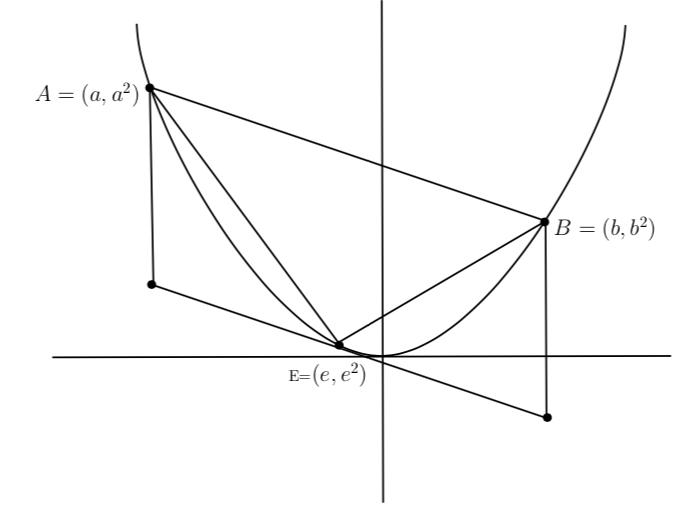
\includegraphics[width=0.4\textwidth]{figures/3.png}
		\end{figure}

		Use this to explain why $\frac{1}{2} \mathcal{A} < \text{area}(\triangle ABE) < \mathcal{A}$.

		\begin{proof}[Solution]
		Let $R$ be the region bounded above by chord $AB$ and below by the parabola $y = x^{2}$; we've been saying that $\mathcal{A}$ is the area of $R$.
		Since $\triangle ABE$ is inscribed in $R$, it follows from the axioms of area that $\text{area}(\triangle ABE) < \mathcal{A}$; it remains to show that $\frac{1}{2} \mathcal{A} < \text{area}(\triangle ABE)$.
		The area of the parallelogram is twice the area of $\triangle ABE$, and again by the axioms of area, since R is inscribed in the parallelogram, $\mathcal{A} < \text{area($p-gram$)} = 2 \cdot \text{area}(\triangle ABE)$, thus $\frac{1}{2}\mathcal{A} < \text{area}(\triangle ABE)$, and we have shown $\frac{1}{2} \mathcal{A} < \text{area}(\triangle ABE) < \mathcal{A}$, as desired.
		\end{proof}
		% subsection part_e (end)

		\subsection*{Part (f)}
		Suppose given another chord $CD$ that is parallel to $AB$, as shown here:
		\begin{figure}[h]
		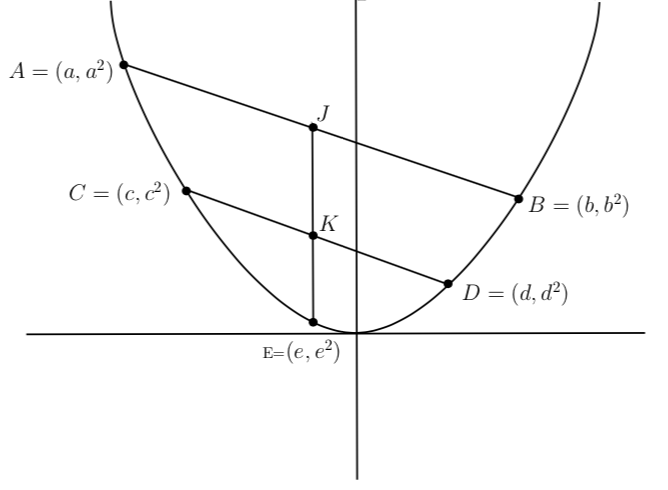
\includegraphics[width=0.4\textwidth]{figures/4.png}
		\end{figure}

		Prove that $\frac{EK}{EJ} = \left( \frac{CK}{AJ} \right)^{2}$.
		(This should remind you a bit of similar triangles, but because we are on a parabola and one edge isn't straight, we get a square on one of the ratios). \dots

		\begin{proof}[Solution]
		Recall that chord $AB$ can be expressed as $y_{1} = x(a+b) - ab$, by similar computations we can express chord $CD$ as $y_{3} = x(c+d) - cd$.
		Further, we have that $e = (a+b)/2 \iff 2e = a+b  \iff b = 2e - a$, thus we can write $y_{1} = (2e)x - a(2e - a)$; and again by similar computations we have $y_{3} = (2e)x - c(2e - c)$.
		The point $J$ is on $y_{1}$ at $x = e$, i.e. for $J = (j,j^{2})$ we have $j = 2e^{2} - 2ae - a^{2}$, so we can write $EJ = 2e^{2} - 2ae - a^{2} - e^{2} = (e-a)^{2}$; by a similar argument we have that $EK = (e-c)^{2}$.
		This allows us to write $$\frac{EK}{EJ} = \frac{(e-c)^{2}}{(e-a)^{2}} = \left( \frac{e-c}{e-a} \right)^{2}.$$
		It remains to show that $CK = e - c$, and $AJ = e - a$.
		\end{proof}
		% subsection part_f (end)
	% section problem_1 (end)

	\section*{Problem 2}
	After the build-up in problem \#1 we are finally ready to get down to business. 
	Start with the chord $AB$, construct the point $E$ as we did in \#1, and draw in the triangle $ABE$. 
	Now do this two more times: once for the chord $AE$ and once for the chord $BE$. 
	In each case we construct the point whose $x$-coordinate is the average of the two next to it. 
	This gives two new triangles, shown in red below:
	\begin{figure}[h]
	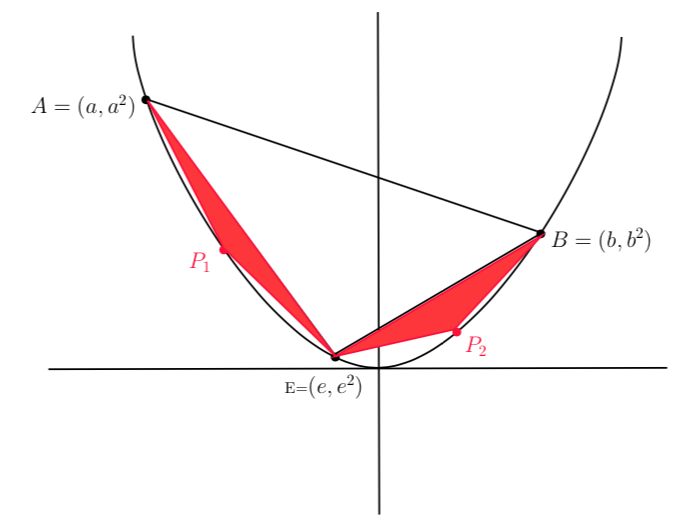
\includegraphics[width=0.4\textwidth]{figures/5.png}
	\end{figure}

	Prove that $\text{area}(\triangle AEP_{1}) = \frac{1}{8} \cdot \text{area}(\triangle AEB)$ by the following argument. 
	Draw the vertical lines $EM$ and $P_{1}M_{1}$, and draw $P_{1}V$ parallel to $AB$ (see picture below). 
	Note that our construction of $P_{1}$ implies that $M_{1}$ is the midpoint of $AM$.
	\begin{figure}[h]
	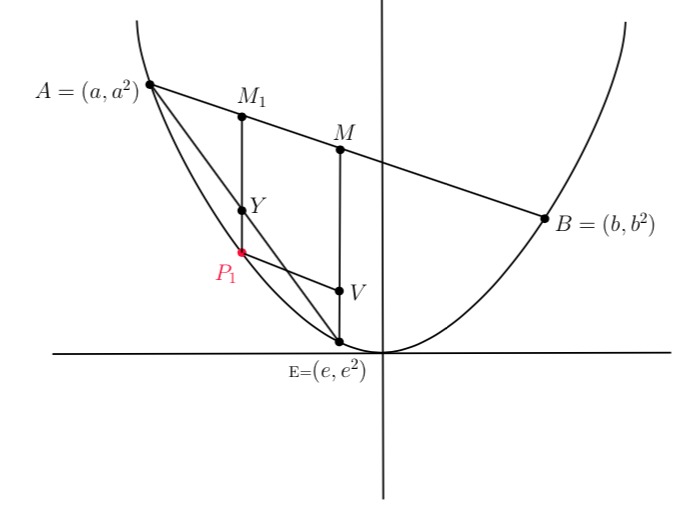
\includegraphics[width=0.4\textwidth]{figures/6.png}
	\end{figure}

	Provide explanations for each step:
		\subsection*{Step 1}
		This follows from \#1f.
		% subsection step_1 (end)

		\subsection*{Step 2}
		Since $M_{1}$ is the midpoint of $AM$, we have that $AM_{1} = M_{1}M = (1/2)AM$, hence $M_{1}M/AM = (1/2)$.
		% subsection step_2 (end)		

		\subsection*{Step 3}
		% subsection step_3 (end)

		\subsection*{Step 4}
		% subsection step_4 (end)

		\subsection*{Step 5}
		% subsection step_5 (end)

		\subsection*{Step 6}
		% subsection step_6 (end)

		\subsection*{Step 7}
		% subsection step_7 (end)

		\subsection*{Step 8}
		% subsection step_8 (end)

		\subsection*{Step 9}
		% subsection step_9 (end)
	Note that the same argument shows that $\text{area}(\triangle BP_{2}E) = \frac{1}{8}\text{area}(\triangle AEB)$.
	% section problem_2 (end)

	\section*{Problem 3}
	Now we do the main analysis of Archimedes.

		\subsection*{Part (a)}
		We started with the ``stage 1'' triangle $\triangle ABE$, then we got two ``stage 2'' triangles $\triangle BEP_{1}$ and $\triangle AEP_{2}$. 
		Continuing in this way, we get four ``stage 3'' triangles, eight ``stage 4'' triangles, and so forth. 
		Let $T_{n}$ be the area of all the stage $n$ triangles taken together. 
		Explain why $$T_{n+1} = k \cdot T_{n}, \hspace{5mm} T_{n} = u_{n} \cdot \text{area}(\triangle ABE)$$ where $k$ and $u_{n}$ are appropriate constants that you provide.

		\begin{proof}[Solution]
		\end{proof}
		% subsection part_a (end)

		\subsection*{Part (b)}
		Next, sum a geometric series to show that $$T_{1} + T_{2} + T_{3} + \cdots = \frac{4}{3}\text{area}(\triangle ABE).$$

		\begin{proof}[Solution]
		\end{proof}
		% subsection part_b (end)

		\subsection*{Part (c)}
		Intuitively it feels like the triangles eventually ``exhaust'' the whole region, and so we have calculated our desired area $\mathcal{A}$. 
		But we have to fully explain this. 
		Let $M_{n} = \mathcal{A} - (T_{1} + T_{2} + \cdots + T_{n})$. 
		This is the area of the ``leftover'' region after all triangles up through stage n have been removed. 
		Problem \#1(e) implies that $T_{n+1} > \frac{1}{2}M_{n}$. 
		Use this to prove that $M_{n+1} < \frac{1}{2}M_{n}$ for all $n$, so that $\lim_{n \to \infty} M_{n} = 0$.

		\begin{proof}[Solution]
		\end{proof}
		% subsection part_c (end)

		\subsection*{Part (d)}
		We have arrived at Archimedes' result that the area of the parabolic region is $\frac{4}{3}$ of the area of the triangle. 
		But carry this one step further and explain why $$\mathcal{A} = \frac{(b-a)^{3}}{6}.$$

		\begin{proof}[Solution]
		Recall that the maximum area of $\triangle ABE$ is $(b-a)^{3}/8$, multiplication by $4/3$ yields that the area of a parabolic region is $(b-a)^{3}/6$.
		\end{proof}
		% subsection part_d (end)
	% section problem_3 (end)

	\section*{Problem 4}
	Redo the area computation from problems \#1-3 using modern integration techniques (like you would do in MATH251). 
	Recall that you wrote down the equation for the line $AB$ in \#1a.

	\begin{proof}[Solution]
	We compute the following:
		\begin{align*}
			\mathcal{A} &= \int_{a}^{b} x(a+b) - ab - x^{2} \ dx, \\
			&= \left( \frac{a}{2}x^{2} + \frac{b}{2}x^{2} - abx - \frac{1}{3}x^{3} \right)\Big|_{a}^{b}, \\
			&= \frac{ab^{2}}{2} + \frac{b^{3}}{2} - ab^{2} - \frac{b^{3}}{3} - \left( \frac{a^{3}}{2} + \frac{a^{2}b}{2} - a^{2}b - \frac{a^{3}}{3} \right), \\
			&= \frac{-ab^{2}}{2} + \frac{b^{3}}{6} - \frac{a^{3}}{6} + \frac{a^{2}b}{2}, \\
			&= \frac{1}{2} \left( a^{2}b - ab^{2} \right) + \frac{1}{6} \left( b^{3} - a^{3} \right), \\
			6 \cdot \mathcal{A} &= 3a^{2}b - 3ab^{2} + b^{3} - a^{3}, \\
			&= (b - a)^{3}, \\
			\mathcal{A} &= \frac{(b - a)^{3}}{6}.
		\end{align*}
	Thus, by simple Riemann integration we have shown that $\mathcal{A} = (b-a)^{3}/6$, which was the final result from Problems \#1-3.
	\end{proof}
	% section problem_4 (end)
\end{document}